\documentclass{report}
\usepackage[utf8]{inputenc}
\usepackage[a4paper]{geometry}
\usepackage{parskip}
\usepackage[acronym,nonumberlist]{glossaries}
\usepackage{tikz}
\usepackage{url}
\usepackage{pgfplots}
\usepackage{titlesec}
\usepackage{tabularx}
\usepackage{array}
\usepackage{arydshln} %Allow dotted lines in tables
\usepackage{graphicx}
\usepackage{wrapfig}
%\pgfplotsset{compat=1.14}

%Changing the Title Format
\titleformat{\chapter}[hang] 
{\normalfont\huge\bfseries}{\thechapter}{1em}{} 
\titlespacing*{\chapter}{0pt}{-50pt}{30pt}

%Adding thick lines for a table
\makeatletter
\newcommand{\thickhline}{%
    \noalign {\ifnum 0=`}\fi \hrule height 1pt
    \futurelet \reserved@a \@xhline
}
\newcolumntype{"}{@{\hskip\tabcolsep\vrule width 1pt\hskip\tabcolsep}}
\makeatother


\makeglossaries

\newacronym{sme}{SME}{small and medium-sized enterprises}
\newacronym{fhtenl}{FHTenL}{Fontys Hogeschool Techniek en Logistiek}
\newacronym{hsnr}{HSNR}{Hochschule Niederrhein}
\newacronym{eu}{EU}{European Union}
\newacronym{mweimh}{MWEIMH NRW}{Ministerium für Wirtschaft, Energie, Industrie, Mittelstand und Handwerk des Landes Nordrhein-Westfalen}
\newacronym{wms}{WMS}{Warehouse Management System}


\author{Lukas Rolle - 2310309}
\title{Project Plan}
\date{\today, Blerick}
\pagenumbering{roman}

\bibliographystyle{abbrv}

\begin{document}
\maketitle
\tableofcontents
\glsaddall

\printglossaries
\listoftables
\listoffigures

\chapter{Introduction}\pagenumbering{arabic}
This document is the project plan for the creation of a demo facility for the LOGwear project.

\section{LOGwear}

\noindent LOGwear is a research project that aims to bring wearables to the area of logistics, especially to \gls{sme}. It is a German-Dutch research project were multiple parties are cooperating to create results. Involved in this are two Universities of applied sciences, \gls{fhtenl} in Venlo as the lead partner, Netherlands and \gls{hsnr} in Krefeld, Germany.

Further on there are also multiple partner companies involved in the project, namely KLG Europe bv, Helmut Beyers GmbH and imat-uve GmbH. These partner companies are there to give the knowledge about logistics processes, as well as to verify and test the results.

The project is backed within the scope of the INTERREG Deutschland-Nederland initiative. It is backed by the \gls{eu}, \gls{mweimh} and the Provincie Limburg as well.



\section{Demo Facility}
The demo facility that should be created for this project will be a physical environment in which a logistics process can be modelled. This process should then be improved by using a wearable. This will be used as a demonstration area for \gls{sme} to see hands-on, if a wearable could be used to improve their own processes. The demo facility will be a proof of concept and not a fully implemented solution that could be directly used at a logistics company and instantly work.

\section{Schedule}
The initial schedule for the project can be seen in table \ref{tab:schedule}. It is to be mentioned, that the schedule is subject to change as the project goes on. The project will be executed in a scrum-like way that is adapted to the group, given the group size of two developers.
\begin{table}[htbp]
\centering
\large
\resizebox{1\textwidth}{!} {
\begin{tabular}{|c"cc:cccc:cc:ccccccccc:ccc:c|} \hline
\textbf{Sprints} & \multicolumn{2}{>{\centering\arraybackslash} m{.15\textwidth}|}{\textbf{Logistics Processes \& Wearables}} & \multicolumn{4}{>{\centering\arraybackslash} m{.35\textwidth}|}{\textbf{Reference Architecture}} & \multicolumn{2}{>{\centering\arraybackslash} m{.25\textwidth}|}{\textbf{Research Demo Facility}} & \multicolumn{9}{c|}{\textbf{Demo Facility Design and Implementation}}                   & \multicolumn{3}{>{\centering\arraybackslash} m{.25\textwidth}|}{\textbf{Creation Demo Facility}} & \multicolumn{1}{>{\centering\arraybackslash} m{.08\textwidth}|}{\textbf{Buf-fer}} \\ \thickhline
Date                 & 06.02              & 13.02              & 20.02                & 27.02                & 06.03         & 13.03        & 20.03        & 27.03 & 03.04 & 10.04 & 17.04 & 24.04 & 01.05 & 08.05 & 15.05 & 22.05 & 29.05 & 05.06         & 12.06        & 19.06        & 26.06                             \\
Week                       & 6                  & 7                  & 8                    & 9                    & 10            & 11           & 12           & 13    & 14    & 15    & 16    & 17    & 18    & 19    & 20    & 21    & 22    & 23            & 24           & 25           & 26 \\\hline       	              
\end{tabular}
}
\caption{Schedule}
\label{tab:schedule}
\end{table}

The schedule is divided in work packages that are to be executed, it is to be noted, that each work package could be split into multiple sprints in the future. In the following subsections the work packages will be explained.

\subsection{Logistics Processes \& Wearables}
This work package includes research about the gives processes and wearables in general, as well as already choosing potential wearables that could be used to improve the process. The end result for this should be a decision on process and wearable. But the result for this could potentially take longer than this task is scheduled. The wearables should be ranked after getting hands-on experience on them, therefore some of them have to be ordered first.

\subsection{Reference Architecture}
A reference architecture should be created for a sample wearable application. What this work package contains is, the creation of diagrams which show the communication from a wearable to the \gls{wms} or something similar. What should not be created is a full reference architecture for a process that is implemented with a concrete wearable. 

It is about creating the always needed layers when using a wearable in a way that supports most wearable solutions.

\subsection{Research Demo Facility}
This task includes researching what physical objects and what systems would be needed to create a demo facility that could showcase a single process with a single wearable. This also includes the gathering of knowledge of where the demo facility should be created and where to get the needed objects.

\subsection{Demo Facility Design and Implementation}
The work package includes the creation of the software design and implementation for the wearable and all aspects that are needed to fully showcase a process.

\subsection{Creation Demo Facility}
This task includes the physical creation of the demo facility. This means setting up shelves with packages to scan and put on a hand pallet truck. Setting up barcodes on the packages to scan. Setting up an environment that can showcase what is happening better to an audience.


\section{Overview}
In this section the following chapters will be shortly explained. 

The first chapter following this, chapter \ref{cha:scope} is about the scope of the assignment. The risk management done in the project will be explained in chapter \ref{cha:riskManagement}. The last chapter will be about the existing stakeholders in the chapter \ref{cha:stakeholders}.
\chapter{Scope}\label{cha:scope}
The scope management is about setting boundaries for the project, which means clearly defining what should be done in the project and, more importantly, what is not part of the project. In section \ref{sec:insideScope} it will be discussed what should be created during the project, while section \ref{sec:outsideScope} is about what should not be created.

\section{Inside of the Scope}\label{sec:insideScope}
\begin{description}
	\item[Reference Architecture] \hfill
	
	A reference architecture for a wearable will be designed and implemented. The reference architecture should allow for simpler future implementations, of applications that should support logistics processes. This reference architecture gives the basic packages that need to exist when working in a wearable in a logistics environment. The reference architecture is given with design, a basic implementation and documentation on different levels of abstractness \cite{Kruchten:1995}.
	\item[Prototype Wearable Application] \hfill
	
	A prototype for a wearable application. It should be a implemented and working solution that is supporting a logistics process. The application is supposed to be a proof on concept.
	\item[Creation Physical Demo Area] \hfill
	
	An area should be rented and prepared to be able to show the prototype application to interested companies. This is intended as a possibility for \gls{sme} to hands-on experience how a wearable could improve their processes.
\end{description}

\section{Outside of the Scope}\label{sec:outsideScope}
\begin{description}
	\item[Finished Product] \hfill
	
	At the end of the project, there should not be a finished product that can be dropped in at any logistics company. Connections to a \gls{wms} or similar should be mocked, but designed to be replaceable to give \gls{sme} a widely usable reference architecture.
	\item[Multiple Demo Scenarios] \hfill
	
	The aim of this project is not to implement multiple demo scenarios, but one more sophisticated process that should be modelled. 
\end{description}
\chapter{Risk Management}\label{cha:riskManagement}
Risk management is about identifying risks and finding solutions to problems before they can occur. The list of risks can be found in table \ref{tab:RiskRegister}. The identified risks will increase as the project moves forward. Especially when a decision is made for the wearable and the process. 

\begin{table}[htbp]
\centering
\footnotesize
\resizebox{\textwidth}{!}{
\begin{tabular}{|p{.03\textwidth}|p{.1\textwidth}|p{.2\textwidth}|p{.08\textwidth}|p{.08\textwidth}|p{.15\textwidth}|p{.13\textwidth}|p{.11\textwidth}|}
\hline
\textbf{Nr} & \textbf{Risk Name}                                    & \textbf{Description}                                                                                                      & \textbf{Prob-ability} & \textbf{Impact} & \textbf{Root Cause}                                                                                       & \textbf{Potential Responses}                                              & \textbf{Risk Owner} \\
\hline
1           & Wearable unavailable          & The wearable desired to be used in the demo facility is unavailable.                                                      & Low                  & Medium          & The desired product is a prototype or similar.                                                            & Choosing a different wearable that is already readily available.          & Graduation Student  \\ \hline
2           & Demo Area & A demo area is in mind that could potentially be rented, but that could not be possible.                                  & Medium               & Medium          & The owner of the place does not rent the area.                                                            & Researching possible places where the demo facility could be created.     & Graduation Student  \\ \hline
3           & Unusable wearable             & A wearable is chosen that does not have the capabilities to fulfill the things that were planned with the demo facility.  & Low                  & High            & Too little research done on the wearables, or the researched material was wrong.                          & Altering the demo scenario to accommodate the problems with the wearable. & Graduation Student  \\ \hline
4           & Vocabulary unclear            & The vocabulary used in the logistics branch, especially abbreviations and acronyms might cause problems in communication. & High                 & Low             & The graduation student has too little knowledge of the logistics branch, at the beginning of the project. & Asking questions if a word's or sentence's meaning is not clear.          & Graduation Student. \\ \hline
\end{tabular}
}
\caption{Risk Register}
\label{tab:RiskRegister}
\end{table}

\begin{wrapfigure}{l}{0pt}
	\centering
	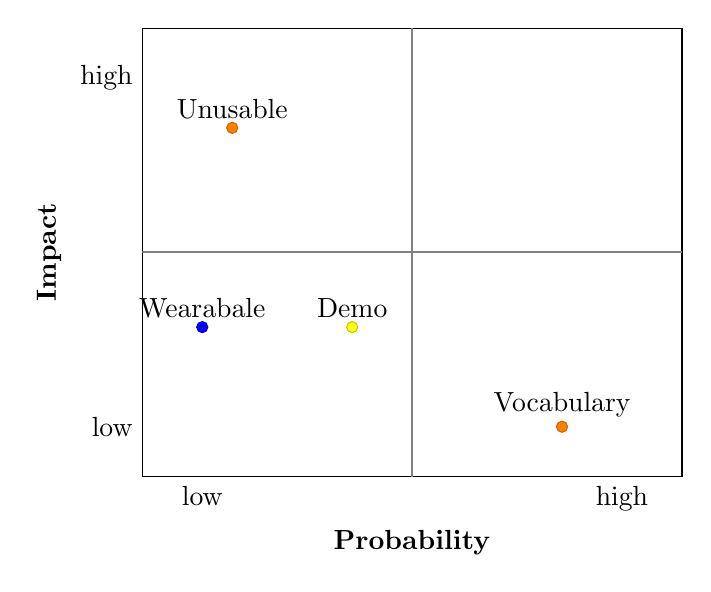
\begin{tikzpicture}
		\begin{axis}[
			scale=1,
			xmin=1,
			xmax=10,
			ymin=1,
			ymax=10,
			xtick,
			ytick,
			extra x ticks={2,9},
  			extra x tick labels={low, high},
  			xtick style={draw = none},
  			extra y ticks={2,9},
  			extra y tick labels={low, high},
			ytick style={draw = none},			
			xlabel=\textbf{Probability},
			ylabel=\textbf{Impact},
			x
			]
			\addplot[
			scatter,
			only marks,
			nodes near coords*={\myvalue},  
			point meta=\thisrow{color},
			visualization depends on={value \thisrow{myvalue} \as \myvalue},
			] table[x=x, y=y]
			{
			x	y	color	myvalue
			2	4	1	Wearabale
			4.5	4	2	Demo
			2.5	8	3	Unusable
			8	2	3	Vocabulary
			0	0 	4
			};
			\addplot[gray,thick, no markers] coordinates {(1,5.5) (10,5.5)};
			\addplot[gray,thick, no markers] coordinates {(5.5,1) (5.5,10)};
		\end{axis}
	\end{tikzpicture}
	\caption{Risk Graph}
	\label{fig:risks}
\end{wrapfigure}

In figure \ref{fig:risks} the risks can be seen in a graph that shows their Probability and Impact again. The color emphasizes the amount of attention a risk should get, in order for the project to continue smoothly.

\chapter{Stakeholders}\label{cha:stakeholders}
Stakeholder Management involves identifying parties that are involved in the project. This ranges from people that are actively part of the development of the project or companies that might be interested in the end result. In the table \ref{tab:stakeholder} the most important stakeholders can be found. The stakeholders will themselves will be further explained in sections \ref{sec:internalStakeholders}, which will explain the internal stakeholders, and \ref{sec:externalStakeholders} will explain the external stakeholders involved in the project.
\begin{table}[htbp]
\centering
\resizebox{\textwidth}{!}{
\begin{tabular}{|p{.04\textwidth}|p{.22\textwidth}|p{.115\textwidth}|p{.118\textwidth}|p{.1\textwidth}|p{.085\textwidth}|p{.16\textwidth}|}
\hline
\textbf{Nr} & \textbf{Stakeholder} & \textbf{Company / Institution} & \textbf{Internal / External} & \textbf{Level of Interest} & \textbf{Level of Influence} & \textbf{Potential management strategies} \\ \hline
1  & Employer             & \gls{fhtenl}        & Internal            & Medium            & High               & Keep Satisfied            \\ \hline
2  & Student Workers      & \gls{fhtenl}        & Internal            & Medium            & Low                & Keep Informed             \\ \hline
3  & Graduation Student   & \gls{fhtenl}        & Internal            & High              & High               & Key Player                \\ \hline
4  & Project Manager      & \gls{fhtenl}        & Internal            & High              & High               & Key Player                \\ \hline
5  & Company Supervisor   & \gls{fhtenl}        & Internal            & High              & High               & Key Player                \\ \hline
6  & Project Team         & \gls{fhtenl}        & Internal            & High              & High               & Key Player                \\ \hline
7 & Partner University   & \gls{hsnr}          & External            & Medium              & Low                & Keep Informed             \\ \hline
8  & Pilot Company        & KLG                   & External            & High              & High               & Key Player                \\ \hline
9  & Examiner             & \gls{fhtenl}        & External            & Low               & High               & Keep Satisfied            \\ \hline
10  & Supervising Lecturer & \gls{fhtenl}        & External            & Medium            & Low                & Keep Informed             \\ \hline
\end{tabular}
}
\caption{Stakeholder Register}
\label{tab:stakeholder}
\end{table}

Figure \ref{fig:stakeholder} can be used to visualize the importance of the stakeholders. The color is used to emphasize the importance that this stakeholder is properly managed.

\begin{figure}[htbp]
	\centering
	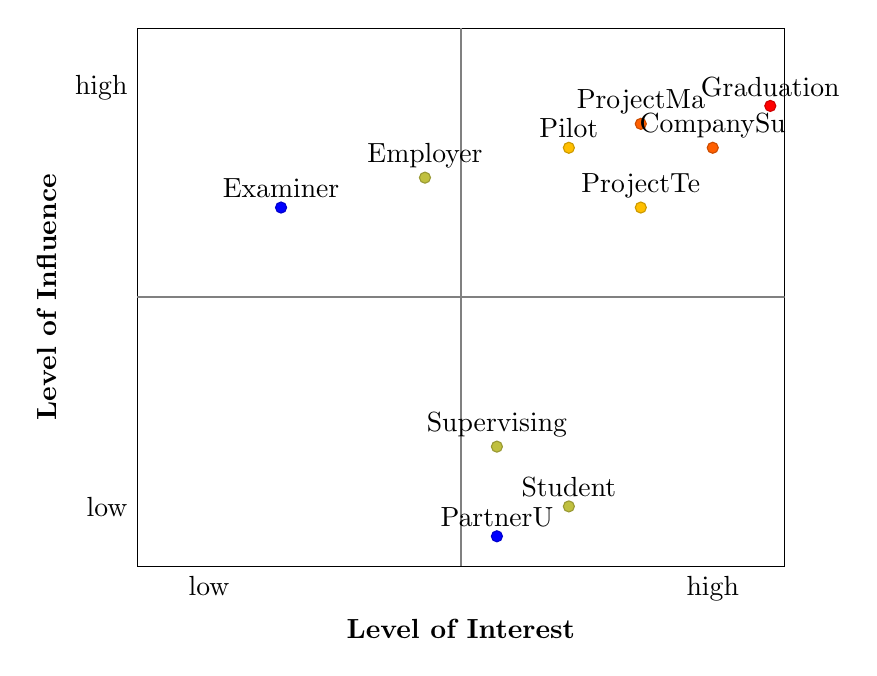
\begin{tikzpicture}
		\begin{axis}[
			scale=1.2,
			xmin=1,
			xmax=10,
			ymin=1,
			ymax=10,
			xtick,
			ytick,
			extra x ticks={2,9},
  			extra x tick labels={low, high},
  			xtick style={draw = none},
  			extra y ticks={2,9},
  			extra y tick labels={low, high},
			ytick style={draw = none},
			xlabel=\textbf{Level of Interest},
			ylabel=\textbf{Level of Influence},
			x
			]
			\addplot[
			scatter,
			only marks,
			nodes near coords*={\myvalue},  
			point meta=\thisrow{color},
			visualization depends on={value \thisrow{myvalue} \as \myvalue},
			] table[x=x, y=y]
			{
			x	y	color	myvalue
			5	7.5	2	Employer
			7	2	2	Student Workers
			7	8	3	Pilot Company 
			3	7	1	Examiner
			6	3	2	Supervising Lecturer
			9.8	8.7	5	Graduation Student 
			8	8.4	4	ProjectMa 
			9	8	4	CompanySu 
			8	7	3	ProjectTe 
			6	1.5	1	PartnerU
			};
			\addplot[gray,thick, no markers] coordinates {(1,5.5) (10,5.5)};
			\addplot[gray,thick, no markers] coordinates {(5.5,1) (5.5,10)};
		\end{axis}
	\end{tikzpicture}
	\caption{Stakeholder Graph}
	\label{fig:stakeholder}
\end{figure}
\section{Internal Stakeholders}\label{sec:internalStakeholders}
Internal Stakeholders are parties that are a part of the team that is working directly on the project in one way or the other. In this section, the internal stakeholders mentioned in table \ref{tab:stakeholder} will be listed again and explained.

\begin{description}
	\item[Employer] \hfill
	
	The employer in this project is an institution and not a single person. This does not change the fact, that the employer is interested in the project, as he is financing the project. Also the employer could change the outcome, if he is not accepting the proposed plans. It is important, that this party is kept satisfied as more work could be created when the plan has to change.
	\item[Student Workers] \hfill
	
	Student Workers are employed to help in the LOGwear project in general. While they currently are not involved with the process of the creation of the demo facility that might change in the future, therefore they should be kept informed.
	\item[Graduation Student] \hfill
	
	The graduation student is the person mainly responsible for the development of the demo facility and therefore has a lot of responsibility and interest towards the project.
	\item[Project Manager] \hfill
	
	The project manager is responsible for the general planning of the project. Planning meetings with the different parties and coordinating them.
	\item[Company Supervisor] \hfill
	
	The company supervisor is looking over the progress of the graduation student and is giving advice if needed. 
	\item[Project Team] \hfill
	
	The project team are the members of the team actively developing the application prototype and are involved in building the demo facility afterwards.
\end{description}

\section{External Stakeholders}\label{sec:externalStakeholders}
External Stakeholders are parties that are involved in the project, but are not a part of the team actively developing the project. In this section, the external stakeholders mentioned in table \ref{tab:stakeholder} will be listed again and explained.

\begin{description}
	\item[Partner University] \hfill
	
	The partner university is also working on the LOGwear project, but on a different aspect. They might be interested in project of creating a demo facility, but probably will not interfere with it.
	\item[Pilot Company] \hfill
	
	The pilot company involved is the logistics company KLG. They bring in the highest amount of domain knowledge and are interested in the project to improve their own processes. They could influence the project easily by not approving the planned demo facility due to problems with how the logistics process is modelled.
	\item[Examiner] \hfill
	
	While the examiner is not involved in the project itself, the examiner will finally assesses the performance of the graduation student.
	\item[Supervising Lecturer] \hfill
	
	The supervising lecturer is there to answer questions and support the student from a software engineering standpoint. While not having a lot of influence on the project itself, the supervising lecturer is interested in what the student is doing and especially how he is doing it.
\end{description}
%\chapter{Initial Analysis}
The process that has been decided on is the Order Picking W3-5. The available Processes were:
\begin{itemize}
	\item Order Picking High Rack
	\item Order Picking W3-5
	\item Goods Receipt and Put away
\end{itemize}

The other two processes were discarded. Order Picking High Rack has been discarded due to the nature of what should be created. A simulation that should model a real environment. Modelling a High Rack and usage of that would be too hard and would take too much time. 

Goods Receipt and Put away Has nothing to do in the Project Plan

\bibliography{99-bibliography}


\end{document}
